\chapter{Technische Unterschiede zwischen Xamarin.Forms und Flutter}
\label{chap:CrossPlattformFrameworks}

Die Unterschiede zwischen den Frameworks werden im folgenden genauer betrachtet.  Für den technischen Vergleich dient Xamarin.Forms als Grundlage.  Die Namen von Abschnitten und Unterabschnitten orientieren sich deshalb an dessen Terminologie.  In den jeweiligen Gliederungspunkten wird anschließend genauer betrachtet,  wie sich spezielle Arbeitsweisen oder Darstellungsoptionen in Flutter abbilden lassen. 

\section{Projektaufbau}
Xamarin.Forms weißt eine andere Projektstruktur auf als Flutter,  das nur mit einem Projekt arbeitet.  Wärend das Flutter Projekt alle notwendigen Inhalte für iOS und Android inkludiert, \footcite[Vgl.][S. 113]{Biessek2019} setzt sich die Projektmappe bei Xamarin.Forms aus mehreren Projekten zusammen.  Es gibt für jede Plattform ein dediziertes Projekt, dass den plattformspezifischen Code,  Konfigurationen und Icons beinhaltet, sowie ein Projekt für den plattformunabhängigen Quelltext.   \footcite[Vgl.][S. 25f.]{Petzold2016} Icons und Konfigurationen werden bei Flutter in einem gleichen oder ähnlichen Format und nur in einem anderen Projekt hinterlegt und lassen sich folglich migrieren.  In den Ausschlusskriterien in Kapitel \ref{chap:CompilerEntwurf} dieser Arbeit wurde bereits der plattformspezifische Quelltext von Xamarin.Forms für die Übersetzung exkludiert.  
\section{Ansichten}
Ansichten (engl. Views) sind visuelle Elemente, die in zwei Kategorien unterschieden werden können.  Steuerelemente (engl. Controls) sind für die Sammlung von Benutzereingaben oder die Ausgabe von Daten verantwortlich und Layouts, beinhalten eine Sammlung von Ansichten und sind für ihre visuelle Anordung auf der Benutzeroberfläche verantwortlich.  \footcite[Vgl.][Abgerufen am \today]{Ritscher2020}

\subsection{Layouts}
Ähnlich wie die Ansichten lassen sich auch die Layouts in zwei Kategorien unterteilen.  Den Ansichtsseiten (engl. Pages) sowie den generellen Layouts. 
Die Pages nehmen den gesamten Bildschirm ein und werden in Abbildung \ref{fig:Xamarin.Forms Pages} dargestellt.\footcite[Vgl.][Abgerufen am \today]{MicrosoftXamPages2016}  

\begin{figure}[!ht]
 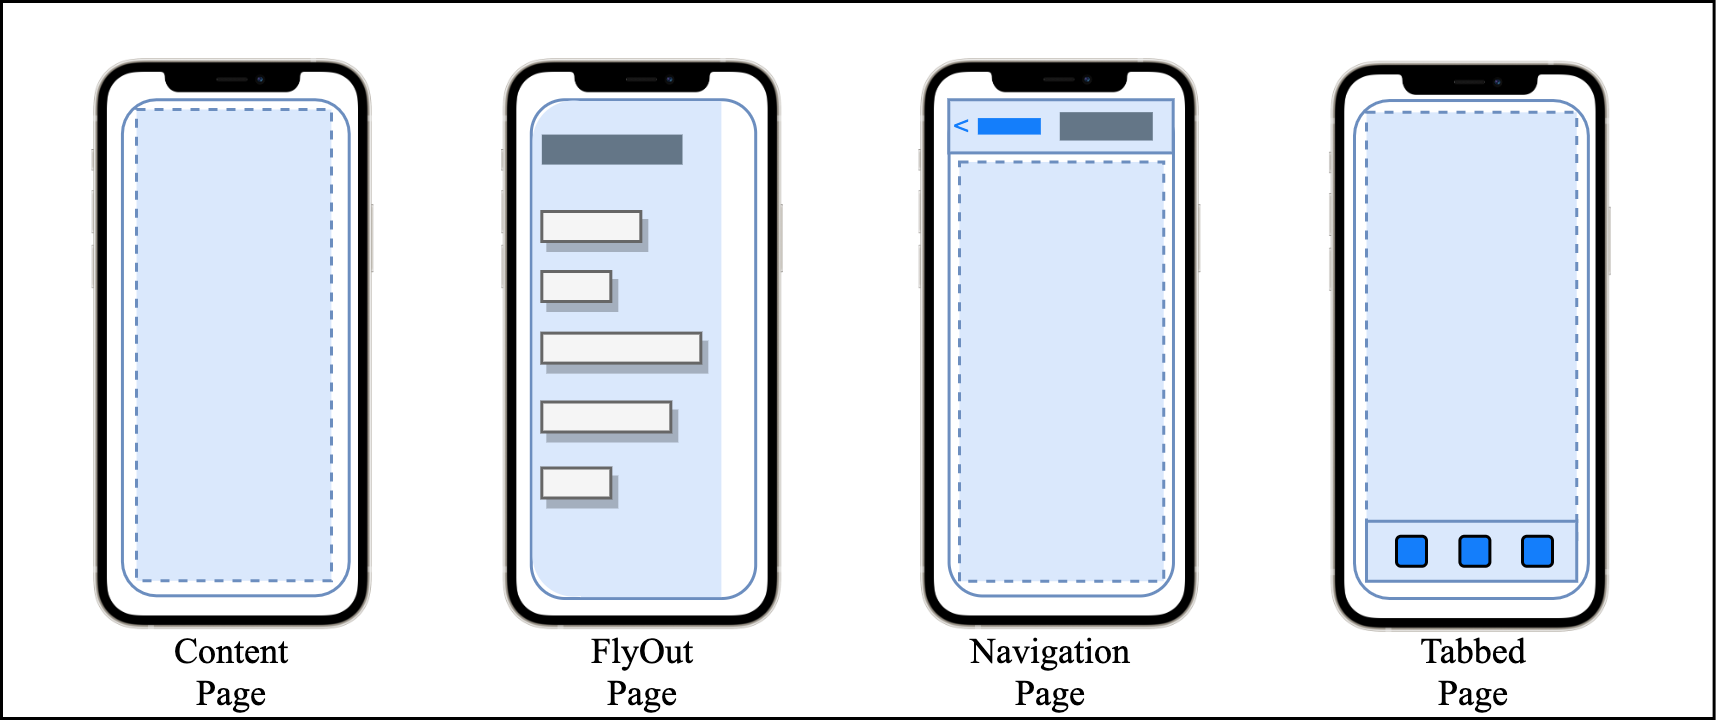
\includegraphics[width=\textwidth,height=\textheight,keepaspectratio]{Images/CrossPlattformFrameworks/XamarinFormsPages.png}
 \caption[Xamarin.Forms Pages]{Xamarin.Forms Pages\footcite{MicrosoftXamPages2016}}
 \label{fig:Xamarin.Forms Pages}
\end{figure}

\glq ContentPage \grq{} ist ausschließlich für die Anzeige einer weiteren Ansicht verantwortlich.  Die drei anderen Pages besitzen ein Navigationskonzept.  \footcitetext[Abbildung in Anlehnung an ][Abgerufen am \today]{MicrosoftXamPages2016} \glq FlyOutPage\grq{} teilt den Bildschirm in zwei Bereiche, ein Bereich dient der Navigation.  Er enthält ein Menü das, wie im Namen enthalten, einfliegen kann.  Der zweite Bereich zeigt eine Detailansicht,  in welcher der Inhalt der angeforderten Seite geladen wird.  \glq NavigationPage\grq{} bietet eine Navigationsleiste, die einen Titel der aktuellen Seite und eine Navigationsschaltfläche beinhalten kann.  \glq TabbedPage\grq{} stellt die unterschiedlichen Seiten als Registerkarten dar. \footcite[Vgl.][Abgerufen am \today]{MicrosoftXamPages2016}
Die Ansichtsseiten befinden sich in der Regel, innerhalb der \ac{xaml}-Datei, auf der untersten Ebene, dem so genannten Wurzelknoten. Der Quelltext \ref{lst:TabbedPage} zeigt dies exemplarisch für eine \glq TabbedPage\grq{} dargestellt,  angegeben.  

\lstinputlisting[label={lst:TabbedPage},caption={[Xamarin.Forms \glq TabbedPage\grq{} Definition]{Xamarin.Forms \glq TabbedPage\grq{} Definition\footcite[Quelltext in Anlehnung an][Abgerufen am \today]{MicrosoftXamTabbedView2020}}} , language=XML]{SourceCode/XamarinFormsTabbedPage.XAML}

Es wird eine \glq TabbedPage\grq{} mit drei Registerkarten entworfen.  Eine Kombination mehrerer Navigationskonzepte ist  möglich,  das Beispiel zeigt eine Navigationsleiste innerhalb der Registerkarten. 

Die verfügbaren Eigenschaften der Ansichtsseiten unterscheiden sich je nach Einsatzszenario.  Im folgenden Quelltext \ref{lst:FlyOutPage} wird dies exemplarisch an der Realisierung einer \glq FlyoutPage\grq{} deutlich.  Anders als bei \glq TabbedPage\grq{}, die aus einer Sammlung von Registerkarten besteht, finden sich im Quelltext die Eigenschaften \glq Flyout\grq{}  und \glq Detail\grq{}.

\lstinputlisting[label={lst:FlyOutPage}, caption={[Xamarin.Forms \glq FlyoutPage\grq{} Definition]{Xamarin.Forms \glq FlyoutPage\grq{} Definition\footcite[Quelltext in Anlehnung an][Abgerufen am \today]{MicrosoftXamFlyOutPage2020}}} ,language=XML]{SourceCode/XamarinFormsFlyoutPage.XAML}

Im Unterschied zu Xamarin.Forms kann Flutter auf der Wurzelebene nur den Style der App,  nicht aber ein Navigationskonzept definieren.  Wie bereits in Kapitel \ref{chap:CompilerEntwurf} aufgeführt, wird in dieser Arbeit ausschließlich der Material Design Style unterstützt. \footcite[Vgl.][Abgerufen am \today]{FlutterForXFDevs} Quelltext \ref{lst:MaterialApp} zeigt die Realisierung einer MaterialDesign App in Flutter.

\lstinputlisting[label={lst:MaterialApp}, caption={[Flutter \glq MaterialApp\grq{} Definition]{Flutter \glq MaterialApp\grq{} Definition\footcite[Quelltext in Anlehnung an][Abgerufen am \today]{GoogleFlutterFirstApp2020}}}, language=Dart]{SourceCode/MaterialApp.Dart}

Der Vergleich zwischen den \ac{xml} basierten \ac{xaml}-Dateien und den bei Flutter verwendeten Dart-Dateien verdeutlicht die Unterschiede in den verwendeten Sprachen zur Benutzeroberflächenentwicklung. 

Die zentrale Idee hinter dem Flutter-Framework ist es,  eine Benutzeroberfläche aus Widgets aufzubauen.  Diese beschreiben das Aussehen der Anwendung basierend auf ihrem aktuellen Zustand.  Sobald sich der Status ändert, kann das Framework den neuen mit dem alten vergleichen, um grafische Veränderungen möglichst effektiv vorzunehmen. \footcite[Vgl.][Abgerufen am \today]{GoogleWidgets2020} Damit in Flutter ein Navigationskonzept definiert werden kann,  können verschiedene Widgets verwendet und verschachtelt werden,  wie in Quelltext \ref{lst:FlutterTabbedApp} beispielhaft für eine App mit Registerkarten visualisiert wird.

\lstinputlisting[label={lst:FlutterTabbedApp},caption={[Flutter \glq Tab Layout\grq{} Definition]{Flutter \glq Tab Layout\grq{} Definition\footcite[Quelltext in Anlehnung an][Abgerufen am \today]{GoogleFlutterTabs2020}}}, language=Dart]{SourceCode/TabbedPage.Dart}

Die deutlichen Unterschiede bei der Auswahl eines Navigationkonzeptes können dadurch überbrückt werden, dass man zu jeder Xamarin.Forms Page das entsprechende Flutter Widget findet.  Der Flutter-Widgetkatalog\footcite[Vgl.][Abgerufen am \today]{GoogleFlutterWidgetCatalog2020} und die Webseite "Flutter for Xamarin.Forms Developers"\footcite[Vgl.][Abgerufen am \today]{FlutterForXFDevs} wurde für die Recherche des Gegenstückes verwendet.  Entsprechende Ergebnisse der Suche können in Tabelle \ref{tab:CompareXFFlutter} abgelesen werden. 


\begin{table}[!ht]
\begin{tabularx}{\textwidth}{X|X}
   \textbf{Xamarin.Forms Page} & \textbf{Flutter Widget}  \\
\hline
	ContentPage            &           	\\ 
	FlyOutPage             & MasterDetailScaffold          	\\ 
	NavigationPage       & Scaffold         	 					\\ 
	TabbedPage            & TabBar und TabBarView 		\\ 
\end{tabularx}
\caption{Gegenüberstellung Pages}
 \label{tab:CompareXFFlutter}
\end{table}
Gegenüberstellungen,  in Tabellenform,  von Xamarin.Forms Elementen und Flutter Widgets werden auch an anderer Stelle in diesem Kapitel der Übersichtlichkeit halber verwendet.  Flutter Widgets die nicht im Text expliziert aufgeführt werden,  sind den Xamarin.Forms Elementen bei Funktionalität und Aussehen nahezu identisch.  Eine vollständige Referenztabelle die sich aus allen Einzelbetrachtungen zusammensetzt, befindet sich in \ref{chap:Gegenueberstellung}. 

Neben den Ansichtsseiten bietet Xamarin.Forms weitere Layouts,  die Steuerelemente zu visuellen Strukturen zusammenstellen.  Abbildung \ref{fig:Xamarin.Forms Layouts} stellt die gebräuchlichsten dieser Layouts vor. 

\begin{figure}[!ht]
 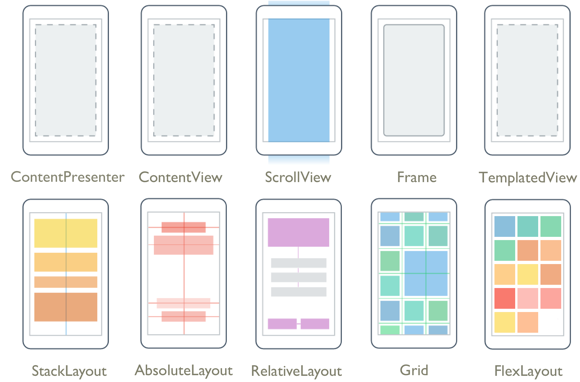
\includegraphics[width=\textwidth,height=\textheight,keepaspectratio]{Images/CrossPlattformFrameworks/XamarinFormsLayouts.png}
 \caption[Xamarin.Forms Layouts]{Xamarin.Forms Layouts\footcite{MicrosoftXamViews2020}}
 \label{fig:Xamarin.Forms Layouts}
\end{figure}

Die vorgestellten Layouts haben  unterschiedliche visuellen Eigenschaften und dienen als Sprachelemente von \ac{xaml} für den Entwurf von Benutzeroberflächen.  \footcitetext[Abbildung in Anlehnung an ][Abgerufen am \today]{MicrosoftXamLayouts2018} \glq ContentView\grq{} enthält ein einzelnes untergeordnetes Ansichtselement und wird als Basisklasse für benutzerdefinierte Darstellungen verwendet.  Das Gestaltungselement \glq StackLayout\grq{} legt untergeordnete Elemente in einem entweder horizontal oder vertikal angeordneten Stapel ab.  Ein \glq Grid\grq{} positioniert seine untergeordneten Elemente in einem Raster aus Zeilen und Spalten,  es wird auch dafür verwendet Layouts und Steuerelemente aufeinander zu legen.  Das \glq ScrollView\grq{} erlaubt das Verschieben von Bildschirminhalten und hat wie ein \glq ContentView\grq{} nur ein untergeordnetes Element.  
Neben diesen gängigen Layouts gibt es noch weniger verbreitete,  zum Beispiel  das \glq  Frame\grq{}, das einen Rahmen um ein visuelles Element zeichnet.  Das \glq AbsolutLayout\grq{},  platziert untergeordnete Elemente an bestimmten Positionen relativ zu ihrem übergeordneten Element und das \glq RelativeLayout\grq{} übernimmt die gleiche Aufgabe jedoch nur auf der Ebene des Layout und untergeordneter Elemente. \footcite[Vgl.][Abgerufen am \today]{MicrosoftXamLayouts2018}

Basierend auf diesen verfügbaren Layouts werden in Tabelle \ref{tab:XamLayouts}  die es entsprechende Flutter Widgets entgegengesetzt.  

\begin{table}[!ht]
\begin{tabularx}{\textwidth}{X|X}
   \textbf{Xamarin.Forms Layout} & \textbf{Flutter Widget}  \\
\hline
	AbsolutLayout       		&  Positioned	 			\\ 
	ContentView       		&  StatelessWidget	 			\\ 
	Frame       					&  BoxDecoration     	 			\\ 
	Grid            				&  GridView oder Stack		\\ 
	ScrollView            		&  SingleChildScrollView		\\ 
	StackLayout       		&  Row und Column  	 			\\ 
	ReleativLayout           &  Positioned		\\ 

\end{tabularx}
\caption{Gegenüberstellung Layouts}
 \label{tab:XamLayouts}
\end{table}

Widgets haben zum Teil erweiterte,  oder abweichende Funktionalitäten, sodass Optimierungen durch den Compiler notwendig sind.  Damit das Layout \glq Grid\grq{} in Xamarin.Forms die Möglichkeit für einen Bildlauf bekommt, weil der Inhalt zu groß für die Darstellung auf einer Seite ist, wird das \glq Grid\grq{} in einem \glq ScrollView\grq{} verschachtelt. Dagegen bietet das \glq GridView\grq{} Widget von Flutter die Option des Scrollens automatisch an, wenn der Inhalt den sichtbaren Bereich überschreitet. \footcite[Vgl.][Abgerufen am \today]{GoogleFlutterGridView2020} Im Rahmen der Codeoptimierung muss das \glq ScrollView\grq{} in diesem Anwendungsfall entfernt werden.

\subsection{Steuerelemente}

Steuerelemente sind die sichtbaren Bausteine der Benutzeroberflächen,  beispielsweise Schaltflächen, Beschriftungen und Textfelder.  
Microsoft kategorisiert die Steuerelemente innerhalb der Frameworkdokumentation anhand ihrer primären Verwendung. \footcite[Vgl.][Abgerufen am \today]{MicrosoftXamViews2020} Diese Einteilung wird folgend übernommen,  obwohl eine klare Abgrenzung der  Steuerelemente zu Kategorien nicht uneingeschränkt möglich ist,  da einzelne zu mehreren Gruppierungen passen.


\subsubsection{Steuerelemente für die Präsentation}
Einige Steuerelemente sind ausschließlich für die Darstellung von Inhalten vorgesehen.  In Xamarin. Forms gibt es die folgenden  Darstellungssteuerelemente, für die eine Flutter Repräsentation notwendig ist.  Das Steuerelement \glq BoxView\grq{ }zeigt in Xamarin.Forms ein einfarbiges Rechteck an.  Für die Darstellung von Texten wird auf \glq Label\grq{} zurückgegriffen.  Bilder können mit Hilfe des \glq Image\grq{}  Steuerelement angezeigt werden,  wobei diese aus verschiedenen Quellen, wie dem Web oder aus den Ressourcen der App geladen werden können.  Das Steuerelement \glq Map\grq{}  kann für die Anzeige von Karten innerhalb der mobilen Anwendung verwendet werden.  Um Web und HTML Inhalte innerhalb einer App visualisieren zu können steht das \glq WebView\grq{}  Steuerelement bereit.  \footcite[Vgl.][Abgerufen am \today]{MicrosoftXamLayouts2018} Für die Steuerelemente kann nun eine Gegenüberstellung zwischen Xamarin.Forms Elementen und Flutter Widgets vorgenommen werden dies wird in Tabelle \ref{tab:ControlsVisualization} dargestellt.

\begin{table}[!ht]
\begin{tabularx}{\textwidth}{X|X}
   \textbf{Xamarin.Forms Steuerelement} & \textbf{Flutter Widget}  \\
\hline
	BoxView		       			&   	 SizedBox  		\\ 
	Image       						&	     Image	 			\\ 
	Label       						&  	Text 					\\ 
	Map            					&	   	Leamaps oder Google Maps \\ 
	WebView            			&  	webview\_flutter	\\ 
	Ellipse							&  	CustomPaint	\\ 
	Linie								&	  	CustomPaint	\\ 
	Path  							&  	CustomPaint	\\ 
	Polygon  						&  	CustomPaint	\\ 
	Polyline und Rectangle  &  	CustomPaint	\\ 
	Rectangle  					&  	CustomPaint	\\ 

\end{tabularx}
\caption{Gegenüberstellung Darstellungssteuerelemente}
 \label{tab:ControlsVisualization}
\end{table}
Zu zeichnende Elemente, wie die  \glq Ellipse\grq{}, \glq Linie\grq{}, \glq Path\grq{},  \glq Polygon\grq{},  \glq Polyline\grq{}  und \glq Rectangle\grq{}wurden nicht besonders aufgeführt,  da diese bei Flutter auf die sogenannte Canvas der Benutzeroberfläche gezeichnet werden können.  \footcite[Vgl.][Abgerufen am \today]{GoogleFlutterCanvas2020} 

\subsubsection{Ereignisauslösende Steuerelemente}
Xamarin.Forms ist ein ereignisgesteuertes Framework. Die hier behandelten Steuerelemente stellen alle mindestens ein Ereignis zur Verfügung,  das mithilfe der in Kapitel \ref{chap:CompilerEntwurf} erwähnten Codebehind Klassen abonniert werden kann.  Sobald ein  sogenanntes Event ausgelöst wird,  übermittelt das Framework diese Information an den Empfänger.   Die folgenden Steuerelemente werden bei Xamarin.Forms dieser Kategorie zugeordnet.  \glq Buttons\grq{} sind rechteckige Objekte,  die einen Text anzeigen und ein \glq clicked\grq{} Ereignis auslösen, nachdem sie von einem Anwender gedrückt wurden.  Mit \glq ImageButton\grq{} steht ebenfalls eine Variante zur Verfügung,  die ein Icon statt einem Text anzeigt.  Bei einem \glq RadioButton\grq{} wird eine Option aus einer Reihe von Möglichkeiten ausgewählt und löst ein Ereignis aus,  wenn sich die Benutzerauswahl ändert.  Ein weiteres Steuerelement ist \glq RefreshView\grq{}, das eine \glq PullToRefresh\grq{}  Funktionalität für Layouts mit Bildlauf anbietet.  Dabei wird durch das Herunterziehen des Seiteninhaltes der Wunsch zur Seitenaktualisierung  übermittelt.  Mithilfe der \glq Searchbar\grq{} haben Anwender die Möglichkeit Inhalte  innerhalb der App zu suchen.  Nach der  Eingabe von Textzeichenfolgen kann per Schaltfläche,  oder Tastaturtaste, ein Ereignis ausgelöst und der eingegeben Text an die Codebehind-Datei weitergeleitet werden.  Tabelle \ref{tab:eventcommands}  zeigt die ereignisauslösenden Steuerelementen von Xamarin.Forms und alternative Flutter Widgets.
\begin{table}[!ht]
\begin{tabularx}{\textwidth}{X|X}
   \textbf{Xamarin.Forms Steuerelemente} & \textbf{Flutter Widget}  \\
\hline
	Button		       				&  	Flatbutton 		\\ 
	ImageButton		       		&  	IconButton 		\\ 
	RadioButton		       		&  	RadioButton 		\\ 
	RefreshView		       		&  	pull\_to\_refresh 		\\ 
	SearchBar		       			&  	flutter\_search\_bar 	\\ 
	SwipeView		       		&  	flutter\_slideable 		\\ 
\end{tabularx}
\caption{Gegenüberstellung ereignisauslösende Steuerelemente}
 \label{tab:eventcommands}
\end{table}

Flutter Widgets verhalten sich nicht exakt gleich wie die Steuerelemente von Xamarin.Forms.  Ein Beispiel ist die hier erwähnte SearchBar, die bei Flutter im Gegensatz zu Xamarin.Forms nicht frei platzierbar ist, sondern immer in der Navigationsleiste angezeigt wird. 

Die Beziehung zwischen Steuerelementen und Codebehind mittels Ereignissen wird  in den beiden folgenden Quelltextausschnitten demonstriert.  Der erste Ausschnitt zeigt  \ac{xaml} Quelltext,  durch welchen ein Button dargestellt werden kann.  Über die Eigenschaft clicked wird auf eine Methode in der XAML.cs Datei verwiesen,  die in dem zweiten Quelltextausschnitt abgebildet ist. 

\lstinputlisting[label={lst:XFVuttonDefinition},caption={Xamarin.Forms Button Initialisierung}, language=XML]{SourceCode/XamarinFormsButton.XAML}

\lstinputlisting[label={lst:XFEventHandler},caption={Xamarin.Forms Event Handler}, , language=csh]{SourceCode/EventHandler.cs}

\subsubsection{Steuerelemente zur Textmanipulation}
In Xamarin.Forms stehen die Arbeit mit Texten die Steuerelemente\glq Entry\grq{}für die Eingabe von einzelnen und  \glq Editor\grq{} von mehreren Textzeilen zur Verfügung.  Tabelle \ref{tab:TextWidgets} zeigt die Gegenüberstellung zu Flutter Widgets.  

\begin{table}[!ht]
\begin{tabularx}{\textwidth}{X|X}
   \textbf{Xamarin.Forms Page} & \textbf{Flutter Widget}  \\
\hline
	Entry		       		&  TextField	 		\\ 
	Editor		       	&  TextField	 		\\ 
\end{tabularx}
\caption{Gegenüberstellung textmanipulierender Steuerelemente}
 \label{tab:TextWidgets}
\end{table}
Wie in der Übersicht erkenntlich besitzt Flutter ausschließlich das Widget \glq TextField\grq{} das beide Funktionalitäten der Xamarin.Forms Steuerelemente bündelt.  Standardmäßig bietet das \glq TextField\grq{} Widget die Eingabemöglichkeit für eine Zeile ähnlich dem \glq Entry\grq{} Steuerelement, kann aber durch das setzen einer Eigenschaft erweitern werden.  Dies wird in Quelltext \ref{lst:FlutterTextField} dargestellt.

\lstinputlisting[label={lst:FlutterTextField},caption={TextField mit mehreren Zeilen in Flutter}, language=Dart]{SourceCode/FlutterTextField.Dart}

\subsubsection{Steuerelemente zur Wertsetzung}
Wersetzung bedeutet das Ergänzen von Steuerelmenten mit Eingaben durch den Anwender der App.  Die folgenden Steuerelemente bietet Xamarin.Forms in dieser Kategorie an.  Das \glq CheckBox\grq{}  Steuerelement ermöglicht dem Benutzer die Auswahl eines boole­schen Wertes (wahr, falsch).  Die gleiche Funktionalität, bei einem anderen visuellen Aussehen siehe Abbildung  \ref{fig:SwitchCheckbox},  bietet der \glq Switch\grq{}.  

\begin{figure}[!ht]
 
\includegraphics[width=\textwidth,height=\textheight,keepaspectratio]{Images/CrossPlattformFrameworks/SwitchTextBox.png}
 \caption{Darstellung von den Steuerelementen \glq Switch\grq{} und \glq Checkbox\grq{}}
 \label{fig:SwitchCheckbox}
\end{figure}
Die beiden linken Darstellungen der jeweiligen Steuerelemente zeigen den Zustand mit dem boolschen Wert falsch , die rechten wahr.

Ein  \glq Slider\grq{}  bieten den Anwendern die Option einen Wert aus einem kontinuierlichen Bereich ein \glq Stepper\grq{}  aus einem Bereich von inkrementellen Werten auszuwählen.  Eine Datumsauswahl wird durch das \glq DatePicker \grq{} Steuerelement ermöglicht,  die Zeitauswahl mit \glq TimePicker\grq{}.  Die Tabelle \ref{tab:valuecontrols} zeigt die gewohnte Gegenüberstellung von Xamarin.Forms Steuerlementen zu Flutter Widgets. 

\begin{table}[!ht]
\begin{tabularx}{\textwidth}{X|X}
   \textbf{Xamarin.Forms Page} & \textbf{Flutter Widget}  \\
\hline
	CheckBox		       				&  Checkbox	 		\\ 
	Switch		       					&  Switch	 		\\ 
	Slider		       					&  Slider	 		\\ 
	Stepper		       				&  number\_inc\_dec	 		\\ 
	DatePicker		       			&  TextField mit Funktion		\\ 
	TimePicker		       			&  TextField mit Funktion	 		\\ 
\end{tabularx}
\caption{Gegenüberstellung wertsetzender Steuerelemente}
 \label{tab:valuecontrols}
\end{table}
 
Für die Steuerelemente \glq DatePicker\grq{}  und \glq TimePicker\grq{} steht kein entsprechendes Widget zur Verfügung.  Durch \glq TextField\grq{} und mithilfe einer Fingergeste wird eine Funktion aufgerufen, die den Auswahldialog für Datum und Uhrzeit öffnet und anschließend die Auswahl in das Textfeld einträgt.  Quelltext \ref{lst:FlutterTimePicker} zeigt diese Funktion in Dart am Beispiel einer Zeitauswahl. 
 \newpage
\lstinputlisting[label={lst:FlutterTimePicker},caption={Verwendung von Timepickern in Flutter}, language=Dart]{SourceCode/FlutterTimePicker.Dart}

Die gesetzten Werte können bei Xamarin.Forms aus den Codebehind Klassen abgefragt werden um den Status eines Steuerelementes zu ermitteln.  Das Abrufen von Informationen in Flutter wird von spezialisierten Widgets beispielsweise dem \glq TextEditingController\grq{} durchgeführt.

\subsubsection{Aktivitätsandeutende Steuerelemente}

In mobilen Anwendungen kann es aufgrund der limitierten Hardware Ressourcen und begrenzten Netzwerkanbindung zu zeitaufwendigen Aktionen kommen.  Zur Visualisierung dieser Ladezeit stehen in Xamarin.Forms die folgenden Steuerelemente zur Verfügung.  Der \glq ActivityIndicator\grq{} zeigt durch eine Animation,  dass eine langwierige Aktivität ausführt wird,  die \glq ProgressBar\grq{} kann mittels Ladebalken auch den Fortschritt darstellen.   Die Tabelle \ref{tab:ActivityControls} zeigt die adäquat Flutter Widgets.

\begin{table}[!ht]
\begin{tabularx}{\textwidth}{X|X}
   \textbf{Xamarin.Forms Page} & \textbf{Flutter Widget}  \\
\hline
	ActivityIndicator		       		&  	CircularProgressIndicator 		\\ 
	ProgressBar		       				&  	LinearProgressIndicator 		\\ 
\end{tabularx}
\caption{Gegenüberstellung aktivitätsandeutender Steuerelemente}
 \label{tab:ActivityControls}
\end{table}


\subsubsection{Sammlunganzeigende Steuerelemente}

Xamarin.Forms stellt für die Darstellung von Datensammlungen Steuerelemente zur Verfügung.  \glq CarouselView\grq{}  zeigt eine blätterbare Liste von Datenelementen an.   \glq IndicatorView\grq{}  stellt mithilfe von Indikatoren die Anzahl der Elemente in einer  \glq CarouselView\grq{} dar.   \glq Picker\grq{}  bietet die Möglichkeit eine Auswahl aus einer Sammlung zu entnehmenund anschließend in einem Textfeld auszugeben.   Die Tabelle \ref{tab:Collections} zeigt die entsprechenden Flutter Widgets an.


\begin{table}[!ht]
\begin{tabularx}{\textwidth}{X|X}
   \textbf{Xamarin.Forms Page} & \textbf{Flutter Widget}  \\
\hline
	CarouselView		       		&  	carousel\_slider  		\\ 
	IndicatorView		       		&  	carousel\_slider		\\ 	
	Picker		       					&  	flutter\_material\_pickers		\\ 
	TableView		       				&  	Table		\\ 
\end{tabularx}
\caption{Gegenüberstellung sammlungsanzeigender Steuerelemente}
 \label{tab:Collections}
\end{table}


\subsubsection{Listen}

Listen sind  Steuerelemente und dienen ebenfalls der Anzeige und Interaktion von Sammlungen.  Aufgrund der langsamen Ladezeiten von \glq ListView\grq{} hat Microsoft im Jahre 2019 mit  \glq CollectionView\grq{}  ein zweites optimiertes Steuerelement für die Anzeige von Listen zur Verfügung gestellt.   \glq SwipeView\grq{} erlaubt einzelne Reihen zur Seite zu schieben und darunter liegende Schaltflächen sichtbar zu machen.  Tabelle \ref{tab:Listview} zeigt die Listen und Ihre Gegenstücke aus dem Flutter Framework. 
\begin{table}[!ht]
\begin{tabularx}{\textwidth}{X|X}
   \textbf{Xamarin.Forms Page} & \textbf{Flutter Widget}  \\
\hline
	List		       				&  	List 		\\ 
	CollectionView		       				&  	List 		\\ 
	SwipeView		       		&  	flutter\_slideable 		\\ 
\end{tabularx}
\caption{Gegenüberstellung Listen}
 \label{tab:Listview}
\end{table}

Die Xamarin.Forms \glq ListView \grq{}ermittelt anhand einer Vorlage,  wie eine Zeile dargestellt werden muss.  Jede Reihe die durch den Benutzer ausgewählt wird,  löst ein Ereignis aus.  Um dieses Verhalten in Flutter abzubilden,  wird die Geste des Widgets in der Liste bereitgestellt.  

Damit sich die ListView im Falle von Änderung in der angezeigten Sammlung automatisch aktualisiert, ist es notwendig die Daten in einer \glq ObservableCollection\grq{} vorzuhalten,  da somit die Benutzeroberfläche über Änderungen informiert wird.   Eine  Möglichkeit, die  \glq ListView\grq{} in Flutter zu aktualisieren, besteht darin, eine neue Instanz des Widget zu erstellen und die Daten aus der alten in die neue Liste zu kopieren.  Dieser Ansatz ist zwar einfach umsetzbar, aber für große Datensätze nicht zu empfehlen.  Eine effektive Änderung für dynamische oder umfangreiche Listen ist mit dem ListView.Builder möglich.   

\section{Gesten}
Für die Interaktion mit der Benutzeroberfläche werden Gesten verwendet.  Die Steuerelemente von Xamarin.Forms stellen Ereignisse für die häufig verwendeten Interaktionen bereit wie im Unterpunkt Ereignisauslösende Steuerelemente aufgeführt.  Alternativ kann die Klasse  \glq GestureRecognizer\grq{}  verwendet werden, um seltenere Benutzerinteraktionen auf Ansichten zu erkennen beispielsweise der click auf eine Steuerelement für die Darstellung.  \footcite[Vgl.][Abgerufen am \today]{MicrosoftGesten2020} 
In Flutter gibt es zwei ähnliche Möglichkeiten: Wird die Ereignisserkennung durch das Flutter-Widget z.B. den \glq ElevatedButton\grq{} untersützt kann eine Funktion übergeben werden, indem eine Geste behandelt wird.  Ist keine Ereignisserkennung durch das Widget unterstützt kann es in einem \glq GestureDetector\grq{} verschachtelt werden wie dies im Rahmen des  \glq Timepickers\grq{} in Quelltext \ref{lst:FlutterTimePicker} dargestellt wurde. \footcite[Vgl.][Abgerufen am \today]{GoogleGesture2020} 

\section{Animation}
Gut gestaltete Animationen machen eine Benutzeroberfläche intuitiver, tragen zum eleganten Erscheinungsbild einer ausgefeilten App bei und verbessern das Benutzererlebnis.  \footcite[Vgl.][Abgerufen am \today]{GoogleFlutterAnimations2020} 
Xamarin.Forms enthält eine eigene Animationsinfrastruktur, die für die Erstellung einfacher Bildsequenzen unkompliziert ist, aber auch vielseitig genug, um komplexe Varianten zu erstellen.  Die Klassen zielen auf verschiedene Eigenschaften von visuellen Elementen ab, wobei eine typische Animation eine Eigenschaft schrittweise, von einem Wert zu einem anderen, über einen bestimmten Zeitraum ändert. \footcite[Vgl.][Abgerufen am \today]{Microsoftanimations2020} 
Flutter stehen vielen Animationen,  insbesondere für Material-Widgets, zur Verfügung.  Sie mit den in ihrer Design-Spezifikation definierten Standard-Bewegungseffekten geliefert,  wobei diese Effekte anpassbar sind.\footcite[Vgl.][Abgerufen am \today]{GoogleFlutterAnimations2020} 

\section{Navigation}
\label{sec:nav}

Die Navigation innerhalb der Anwendung hängt bei Xamarin.Forms hauptsächlich von der verwendeten Ansichtsseite und ihrem Navigationkonzept ab.  So bietet die NavigationPage eine hierarchische Navigation, bei der der Benutzer durch die Seiten vorwärts und rückwärts navigieren kann. \footcite[Vgl.][Abgerufen am \today]{MicrosoftXamNavigation2020}   Flutter hat eine ähnliche Implementierung,  die einen Navigator und Routen verwendet.  Route sind  Abstraktionen für die Seiten einer App, und ein Navigator ist ein Widget, das Routen verwaltet.  Der Navigator arbeitet ähnlich wie die Xamarin.Forms NavigationPage, indem er Seiten aufrufen kann abhängig davon ob man zu einer Ansicht hin oder von ihr zurück navigieren möchte.\footcite[Vgl.][Abgerufen am \today]{GoogleFlutterNavigation2020} 


Neben der internen Navigation innerhalb einer Anwendung ist es auch möglich zwischen verschiedenen Apps zu navigieren.  Dafür greift Xamarin Forms auf ein bestimmtes URI-Schema zurück.  Mit dem Befehl Launcher.OpenAsync("mailto://") kann so z.B. das  Standard E-Mail-Programm des Gerätes geöffnet und werden verwenden. \footcite[Vgl.][Abgerufen am \today]{MicrosoftLauncher2020}  In Futter kann für diese Funktionalität mithilfe des Plugins urllauncher Anwendungen hinzugefügt werden.\footcite[Vgl.][Abgerufen am \today]{Googleurllauncher2020} 

\section{Lebenzyklus}
Durch das Navigieren zu anderen Anwendungen ändert sich der Status von im Fordergrund zu im Hintergrund . Der aktuelle Zustand einer App bestimmt, was sie zu jedem Zeitpunkt tun kann und was nicht.  Zum Beispiel hat eine Vordergrund-App die Aufmerksamkeit des Benutzers, also hat sie Vorrang bei de,m Zugriff auf Systemressourcen, einschließlich der CPU.  Im Gegensatz dazu muss eine Hintergrund-App so wenig wie möglich arbeiten, am besten gar nichts, da sie sich außerhalb des Bildschirms befindet.  Wenn eine App ihre Zustand wechselt,  müssen sie ihr Verhalten entsprechend anpassen.\footcite[Vgl.][Abgerufen am \today]{AppleLifecycycle2020} 

Xamarin.Forms bitetet für die Arbeit mit dem Lebenzyklus der App die folgenden drei Methoden \glq OnStart\grq{} , \glq OnResume\grq{}  und \glq OnSleep\grq{} an die aufgerufen werden wenn sich der Status der Anwendung verändert. \footcite[Vgl.][Abgerufen am \today]{MicrosoftXamLifecycle2020} Bei Flutter kann auf die ‚didChangeAppLifecycleState ‘ Methode zurückgegriffen werden, die bei Änderungsereignissen ausgelöst wird und die drei Lebenszyklen beinhaltet. \footcite[Vgl.][Abgerufen am \today]{GoogleFlutterLifeCycle2020} 

\section{Erweiterungen}
Erweiterungen sind Programmergänzungen, die auch von externen Entwicklern beigetragen werden können.  Sie dienen der Reduzierung des Entwicklungsaufwandes, da nicht jede Funktionalität eigens implementiert werden muss.  Im .NET-Ökosystem können Xamarin.Forms-Projekte auf das Paketverwaltungssystem Nuget zurückgreifen,  um Erweiterungen zu einer App hinzuzufügen. \footcite[Vgl.][Abgerufen am \today]{MicrosoftXamNuget2020}  Bei Flutter wird für diesen Fall mit der pubspec.yaml Datei eine Referenz auf das ausgewählte Plugin gesetzt.  Dabei unterscheidet Flutter zwischen Packeten, welches Erweiterungen sind die in Dart geschrieben wurden und Plugins dabei handelt es sich um eine Erweiterung die Plattformfunktionalität verfügbar macht.  Plugins können für Android (mit Kotlin oder Java) oder für  iOS (mit Swift oder Objective-C) geschrieben sein. \footcite[Vgl.][Abgerufen am \today]{GoogleFlutterPackages2020} In Quelltext \ref{tab:Listview} wird ein Auschnitt der pubspec.yaml Datei gezeigt, in welcher das in Abschnitt \ref{sec:nav} erwähnte Plugin für das öffnen von anderen Anwendungen mit Hilfe von URL's als Abhängigkeit geladen wird.

\lstinputlisting[label={lst:Pubspecjaml},caption={[Erweiterungen in Flutter]{Erweiterungen in Flutter\footcite[In Anlehnung an ][Abgerufen am \today]{GoogleFlutterPackages2020}}}, language=Dart]{SourceCode/Pubspec.yaml}
In dem Beispiel muss das Plugin eine mindeste Version von 5.4 haben darf jedoch die Version 6 nicht überschreiten. 

\section{Bilder}
Bilder können in Apps das Benutzererlebnis verbessern und helfen eine Aktion zu veranschaulichen oder komplexe Botschaften verdeutlichen.  \footcite[Vgl.][Abgerufen am \today]{GoogleMaterialImages2020} In iOS und Android können Bilder in verschiedenen Auflösungen bereit gestellt werden,  das Betriebssystem wählt während der Laufzeit das beste Bild basierend auf den Eigenschaften des Smartphonedisplays.  Xamarin.Forms verwendet die \acfp{api} der nativen Plattformen zum Laden lokaler Bilder und unterstützt daher die plattformspezifischen  Funktionalitäten,  wenn die Dateiennamen korrekt sind und sich im Projekt befinden.\footcite[Vgl.][Abgerufen am \today]{MicrosoftXamImages2020} Zur Verwendung nativer Bilddateien müssen die Bilder in Xamarin.Forms zu jedem Anwendungsprojekt hinzugefügt werden und vom gemeinsamen Xamarin.Forms-Code referenziert werden. 

Flutter verwendet Im Gegensatz zu Xamarin.Forms keine nativen \acs{api} sondern verwendet ein einfaches dichte-basiertes Format,  ähnlich dem von iOS.  Für die Anzeige von Bildern verwendet Flutter sogenannte logische Pixel, die im Grunde dasselbe sind wie geräteunabhängige Pixel.  Mithilfe der sogenannte devicePixelRatio kann das Verhältnis von physikalischen Pixeln zu einem einzelnen logischen Pixel ermittelt werden. Bei Flutter können sich alle Bilder in einem beliebigen Ordner befinden da Flutter keine vordefinierte Ordnerstruktur hat. \footcite[Vgl.][Abgerufen am \today]{GoogleFlutterImages2020} 

\section{Schriftsatz}
Ein Schriftsatz wird verwendet um das Design und den Inhalt so klar und effizient wie möglich darzustellen.  In Xamarin.Forms mussten Schriften bis zum Jahre 2020 in jedem nativen Projekt referenziert werden.  Seit der Version 4.5 können Fonts (deutsch Schriftart) jedoch auch zwischen den Plattformen geteilt werden und befinden sich daher innerhalb des geteilten Projektes. \footcite[Vgl.][Abgerufen am \today]{Versluis2020}  In Flutter werden die Schriftdateien ähnlich wie in der neueren Version von Xamarin.Forms in einem Ordner abgelegt. \footcite[Vgl.][Abgerufen am \today]{GoogleFlutterFonts2020}  Eine Verwendung eines bestimmten Schriftsatzes wird in \ref{lst:FlutterFont} dargestellt.  

\lstinputlisting[label={lst:FlutterFont},caption={Flutter Font definition}, language=Dart]{SourceCode/Fonts.Dart}



\section{Interaktion mit der Hardware}
Android und iOS nutzen einzigartige Betriebssystem- und Plattform-\acs{api} , auf die Xamarin.Forms Entwickler zugreifen können.  Mit der Erweiterung Xamarin.Essential bietet Microsoft bietet eine plattformübergreifende \ac{api}, auf die von gemeinsamem Code aus zugegriffen werden kann und direkt auf der Plattform ausgeführt wird.  Der Dart-Code, aus dem eine Flutter-App besteht, wird nativ auf dem Gerät ausgeführt,  zum Beispiel eine Netzwerkanfrage in Dart würde im direkten Dart-Kontext(Umfeld) ausgeführt,  wobei das von der Plattform bereitgestellte \ac{sdk} umgangen wird. Es werden in diesem Fall also nicht die Android- oder iOS-\acs{api}  genutzt.  Das bedeutet, wenn zum Beispiel eine Netzwerkanfrage in Dart durchgeführt wird diese direkt im Dart-Kontext ausgeführt wird.  Es werden also nicht die Android- oder iOS-\acs{api} genutzt.  Das bedeutet aber nicht, dass Flutter-Apps nicht mit diesen nativen \ac{api} oder mit Ihrem nativen Code interagieren können. Flutter bietet sogenannte Plattformkanäle, die mit dem ViewController oder der Activity, die Ihre Flutter-Ansicht hostet, kommunizieren und Daten austauschen. Plattformkanäle sind im Wesentlichen ein asynchroner Messaging-Mechanismus, der den Dart-Code mit dem Host-ViewController oder der Activity und dem iOS- oder Android-Framework, auf dem er läuft, verbindet. Sie können Plattformkanäle verwenden, um eine Methode auf der nativen Seite auszuführen oder um z. B. einige Daten von den Sensoren des Geräts abzurufen.\footcite[Vgl.][Abgerufen am \today]{GooglePlatformspecificCode2020}

\section{Speicherung von Daten}
Ein wesentlicher Bestandteil jeder mobilen Anwendung ist die Fähigkeit,  Daten zu persistieren.  Manchmal handelt es sich dabei um große Datenmengen,  die eine Datenbank erfordern,  oft sind es aber auch kleinere Daten wie Einstellungen und Präferenzen, die zwischen den Starts der Anwendung gespeichert werden müssen.   Die eingeführte Xamarin.Essentials erweiterung stellt Entwicklern das Settingsplugin bereit, welches die Speicherung von Einstellungen in einem Schlüsselwertspeicher erlaubt.  \footcite[Vgl.][Abgerufen am \today]{MicrosoftXamSettings2019} In Flutter wird für die Speicherung von Schlüssel-Wertpaaren auf die gleichen plattformspezifischen \ac{api} zugegriffen wie bei Xamarin Forms diese werden ebenfalls mithilfe eines Plugins angesprochen.  \footcite[Vgl.][Abgerufen am \today]{GoogleFlutterSharedPreferences2020}  Die Verwendung des gleichen Plugins ist ein wichtiger Faktor,  da auf die von Anwendern gespeicherten Schlüsselwert Paaren, auch nach einem Framework Wechsel zu Flutter,  zurückgegriffen werden kann. 

Für die Speicherung in einer Datenbank können Xamarin.Forms Entwickler auf verschiedene Lösungen zurückgreifen zum einen SQLite die am häufigsten verwendete Datenbank-Engine der Welt\footcite[Vgl.][Abgerufen am \today]{SQLiteConsortium2020},  oder Realm einer Datenbank optimiert für mobile Endgeräte. \footcite[Vgl.][Abgerufen am \today]{MongoDBRealm2020} Beide Datenbanken stehen auch als Plugin für Flutter zur Verfügung, wobei SQLite ausgereift ist,\footcite[Vgl.][Abgerufen am \today]{Tekartik2020} während Realm erst am 5 November 2020 support für Flutter angekündigt hat und noch nicht offiziell zur Verfügung steht. \footcite[Vgl.][Abgerufen am \today]{MongoDBFlutterSupport2020}
